\documentclass[reportComp,bib]{thesis}
\usepackage[cpp,linenum]{mypackage}

\title{数值计算方法课题报告}
\subtitle{Algorithm 942: Semi-Stencil}
\school{数据科学与计算机学院}
\author{17341015 陈鸿峥\quad17341111 刘学海\quad17341109 刘佳荣}
\classname{17大数据与人工智能}
\stunum{}
\headercontext{数值计算方法课题报告}

\begin{document}

\maketitle

我们小组选定的论文是
Ra\'ul De La Cruz and Mauricio Araya-Polo, \emph{Algorithm 942: Semi-Stencil}, ACM Transactions on Mathematical Software, Vol.40, No.3, Artical 23, 2014。

下面将阐述该论文的核心内容,以及我们接下来的研究方向。

\section{背景}
\label{sec:bg}
Stencil\footnote{由于在国内没有找到对该词比较好的翻译,故下文依然保留stencil的叫法}广泛应用在各个领域,如图像处理\cite{kernel}、解线性方程组(Gauss-Seidel\cite{gauss-seidel})、有限元分析\cite{fem}、偏微分方程(PDE)\cite{pde}等,因而优化stencil计算的执行时间对于大量的科学应用十分重要。

维基百科上给出的stencil例子\cite{stencil},如图\ref{fig:stencil_example}所示,即一个stencil是一种数组更新的模式(pattern)。
\begin{figure}[H]
\centering
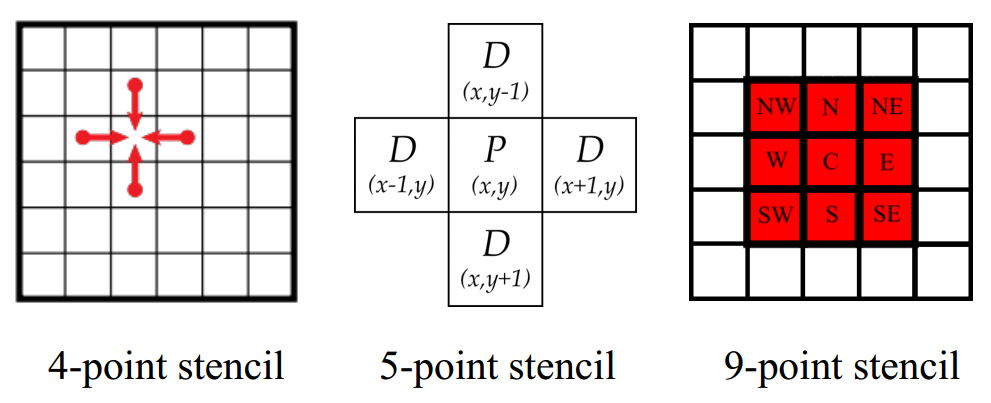
\includegraphics[width=0.6\linewidth]{fig/stencil-example.PNG}
\caption{stencil例子}
\label{fig:stencil_example}
\end{figure}

我们阅读的论文主要针对PDE求解中有限差分方法(Finite Difference, FD)采用的stencil计算进行优化,即只考虑坐标轴方向上的stencil(图\ref{fig:stencil_example}后两者),而不考虑其他方向上的stencil(图\ref{fig:stencil_example}前者,卷积操作)。

\section{问题定义}
\label{sec:problem}
由于原文作者主要以三维空间为例讲述,故这里我们也考虑三维空间的情况,高维空间根据下列定义可同理扩展。

考虑三维空间中的格点$\sX_{i,j,k}^t$,即数组元素\verb'a[i,j,k]'在$t$时刻的值。
参数$l$代表每个方向上需要用访问的邻居(neighbor)个数。

利用该定义给出一个传统的stencil如下,其中$C$为稀疏(discretization)系数,$X,Y,Z$为三个轴
\[\begin{aligned}
\sX_{i,j,k}^t &= C_0*\sX_{i,j,k}^{t-1}\\
&+C_{Z1}*(\sX_{i-1,j,k}^{t-1}+\sX_{i+1,j,k}^{t-1})+\cdots+C_{Zl}*(\sX_{i-l,j,k}^{t-1}+\sX_{i+l,j,k}^{t-1})\\
&+C_{X1}*(\sX_{i,j-1,k}^{t-1}+\sX_{i,j+1,k}^{t-1})+\cdots+C_{Xl}*(\sX_{i,j-l,k}^{t-1}+\sX_{i,j+l,k}^{t-1})\\
&+C_{Y1}*(\sX_{i,j,k-1}^{t-1}+\sX_{i,j,k+1}^{t-1})+\cdots+C_{Yl}*(\sX_{i,j,k-l}^{t-1}+\sX_{i,j,k+l}^{t-1})
\end{aligned}\]
代表的即中心节点通过$X,Y,Z$三个方向上正负半轴各$l$个等距结点来更新。

该文主要解决两个问题:
\begin{enumerate}
	\item 稀疏内存访问模式:\\
在计算机组成原理中我们学过,内存的组织是线性的,按行优先或列优先存储。
比如按照X方向优先存储,那么其他两个方向上的stencil格点虽然在数学坐标系上是相邻的,但在实际存储结构中,它们是分离的。
这就导致现代计算机体系的内存层次结构失效,即cache miss经常会发生,进而需要更多的时间来访问主存。

	\item 低数据重用率导致的低算存比(compute to cache access ratio, CCAR\footnote{这个指标是自己定义的,原文定义太过冗长,CCAR的公式很好理解})
\begin{equation}
\label{equ:ccar}
\begin{aligned}
CCAR&=\frac{\text{Floating Point Op}}{\text{Data Cache Accesses}}=\frac{2*\text{MultiplyAdd Ins}}{\sX^{t-1}\text{Loads}+\sX^{t}\text{Stores}}\\
&=\frac{2*2*\dim*l+1}{(2*(\dim-1)*l+1)+(1)}=\frac{4*\dim*l+1}{2*\dim*l-2*l+2}
\end{aligned}
\end{equation}
只有同一维度方向上的数据可以(在短时间内)被重用,因而大量的数据被重复地读入和写出。
同样,没有很好利用数据的时间局部性,cache失效。
\end{enumerate}

\section{模型分类}
图\ref{fig:catalog}展示的是目前stencil主要做的优化点,可以看到该文作者提出的semi-stencil算法属于无关硬件算法层面的优化。
\begin{figure}[H]
\centering
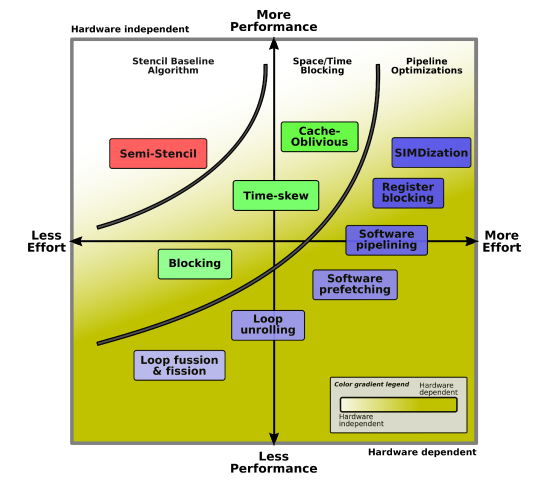
\includegraphics[width=0.5\linewidth]{fig/schemes.PNG}
\caption{目前针对stencil问题方法的分类}
\label{fig:catalog}
\end{figure}

\section{算法}
针对第\ref{sec:bg}节存在的问题,该文作者提出semi-stencil算法。

其算法的核心观点非常简单,即\textbf{通过减少访存次数,提升算存比,以提高并行性,最终获得性能提升}。

Semi-stencil主要包含两个步骤,一个前向(forward)更新,一个后向(backward)更新,如图\ref{fig:forward-backward}所示。
\begin{figure}[H]
\centering
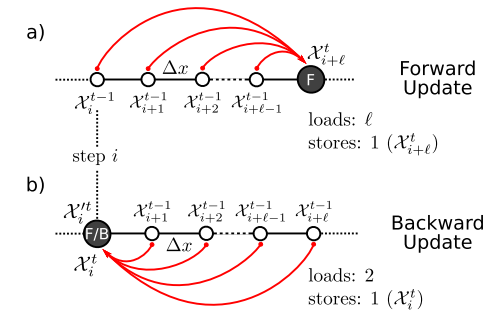
\includegraphics[width=0.5\linewidth]{fig/forward-backward.PNG}
\caption{前向与后向更新}
\label{fig:forward-backward}
\end{figure}

即将原来同一轴正负两侧方向的更新拆开来,每次只做一侧的更新(因而叫semi-stencil),正向称为前向更新,负向称为后向更新。
同时注意到如果前向更新了$i$结点,后向更新相隔$l$个单位的结点,那么数据就可以被重用了,即$i$到$i+l$的部分不用写入主存,直接可以用来计算。

容易算得新的CCAR为
\begin{equation}
CCAR=\frac{\text{Floating Point Op}}{\text{Data Cache Accesses}}=\frac{4*\dim*l+1}{\dim*l-l+2*\dim}
\end{equation}

对比方程\ref{equ:ccar},明显CCAR提升了。

具体实施则是将程序分为三个部分,头部(head)、中部(body)和尾部(tail)。
由于存在内点(interior)和外点(ghost),故需要区别更新策略。
头部只进行前向更新,尾部只进行后向更新,中部则前后向更新都要完成,如图\ref{fig:algorithm}所示。
\begin{figure}[H]
\centering
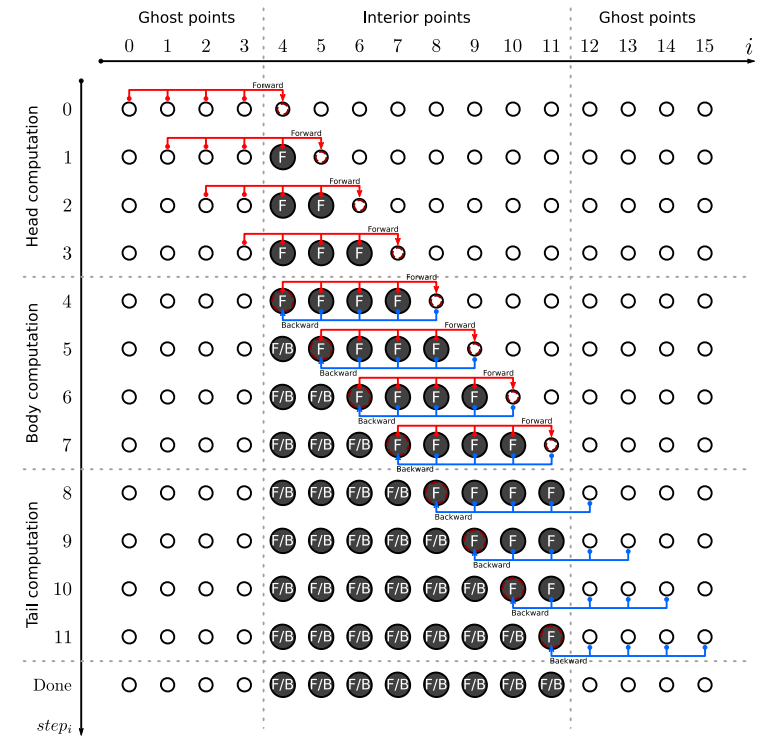
\includegraphics[width=0.5\linewidth]{fig/algorithm.PNG}
\caption{具体算法实施}
\label{fig:algorithm}
\end{figure}

具体算法细节比较冗长,就不贴在这了。
简而言之,该算法将原来单一的嵌套循环,拆分成多个嵌套循环(头部、中部、尾部),每个循环的访存次数少了,进而CCAR提升了;外层的循环没有互相之间的依赖关系,也容易并行,最终性能提升。

\section{实验}
针对4种不同的CPU架构、4种不同的stencil算法、以及不同的stencil大小进行实验。

实验结果如预期,提升了cache命中率,减少了访存次数,进而提升性能。

具体实验结果请见论文原文。
但是很遗憾的是,该文并没有给出它与state-of-the-art算法的比较,用最原始的方法做对比当然能够胜出。

\section{总结与未来研究}
这篇文章虽然发表在2014年,但是它引用做stencil的文章大多都比较老,采用的方法无论是从数学角度还是从计算机角度,都做得太过粗浅。
而且该文章针对的stencil不具有通用性,且只在代码层面进行人工优化,没有实现自动并行。

所以我们在这篇文章的基础上可以做的空间还有很大,我们期望借用semi-stencil的想法,或提出更好的优化方法,进而将stencil的研究扩展到更广阔的领域。

下面列举的内容是之后\textbf{可能}进行研究的方向。
\begin{itemize}
	\item 算法层面优化:
	\begin{itemize}
		\item 将循环体的迭代空间用高维格点数组表示\cite{pouchet:reuse_fpga_2013},通过定义一些线性代数的基本运算,计算量化stencil迭代计算过程中的重用率
		\item 通过一些编译器优化技术(主要是多面体模型\cite{baghdadi:tiramisu_cgo_2019}),进一步优化stencil,并针对stencil重新做评估
	\end{itemize}
	\item 算法实现:
	\begin{itemize}
		\item 在CPU上用OpenMP或Cilk-plus\cite{cellular-automaton}实现并行
		\item 如果有条件用cuda编程上GPU加速
	\end{itemize}
	\item 算法应用:
	\begin{itemize}
		\item 图像处理:前文已经提到stencil在图像处理中大量使用,因此我们打算结合Halide\cite{ragan-kelley:pldi_halide_2013}这一图像流处理语言,将semi-stencil的算法植入其中,并测试端到端的性能
		\item 元胞自动机:其是一种时间、空间、状态都离散,空间相互作用和时间因果关系为局部的网格动力学模型,具有模拟复杂系统时空演化过程的能力。
		容易发现stencil与元胞自动机的高度相关性,利用该论文的semi-stencil的方法,可以使元胞自动机的效率模拟行为的速度进一步提高。
	\end{itemize}
\end{itemize}

\bibliography{nc}

\end{document}
% 课程名称,小组成员(学号姓名),论文标题,科学问题,问题定义,定理,模型,算法,修改应用
% 翻译、总结
% 周二20:00
% 1024180018@qq.com